\documentclass[11pt,a4paper,onside,UTF8]{article}
\usepackage{geometry}
	\geometry{left=2cm,right=2cm,top=2.5cm,bottom=3cm}
\usepackage[utf8]{inputenc}
\usepackage[english]{babel}
\usepackage{lipsum}
\usepackage{bm}
\usepackage{upgreek}

\usepackage{amsmath}
% mathtools for: Aboxed (put box on last equation in align envirenment)
\usepackage{microtype} %improves the spacing between words and letters

\usepackage{xeCJK,paralist,enumerate,booktabs,multirow,graphicx,float,setspace}
	\setlength{\parindent}{2em}%正文首行缩进两个汉字
% \usepackage{ctex}
%     \setmainfont{Times New Roman}

%% COLOR DEFINITIONS

\usepackage[svgnames]{xcolor} % Enabling mixing colors and color's call by 'svgnames'

\definecolor{MyColor1}{rgb}{0.2,0.4,0.6} %mix personal color
\newcommand{\textb}{\color{Black} \usefont{OT1}{lmss}{m}{n}}
\newcommand{\blue}{\color{MyColor1} \usefont{OT1}{lmss}{m}{n}}
\newcommand{\blueb}{\color{MyColor1} \usefont{OT1}{lmss}{b}{n}}
\newcommand{\red}{\color{LightCoral} \usefont{OT1}{lmss}{m}{n}}
\newcommand{\green}{\color{Turquoise} \usefont{OT1}{lmss}{m}{n}}

\DeclareMathOperator{\trace}{trace}
\DeclareMathOperator{\diag}{diag}

%% FONTS AND COLORS

%    SECTIONS

\usepackage{titlesec}
	\newfontfamily\sectionef{Times New Roman}
	\setCJKfamilyfont{FZHeiTi}{黑体}
	\newcommand{\sectioncf}{\CJKfamily{FZHeiTi}}
	\titleformat*{\section}{\large\bfseries\sectioncf\sectionef}
	\titleformat*{\subsection}{\normalsize\bfseries\sectioncf\sectionef}
\usepackage{sectsty}
%%%%%%%%%%%%%%%%%%%%%%%%
%set section/subsections HEADINGS font and color
\sectionfont{\color{MyColor1} \usefont{OT1}{lmss}{b}{n}}  % sets colour of sections
\subsectionfont{\color{MyColor1}\usefont{OT1}{lmss}{b}{n}}  % sets colour of sections

%set section enumerator to arabic number (see footnotes markings alternatives)
\renewcommand\thesection{\arabic{section}.} %define sections numbering
\renewcommand\thesubsection{\thesection\arabic{subsection}} %subsec.num.

%define new section style
\newcommand{\mysection}{
\titleformat{\section} [runin] {\usefont{OT1}{lmss}{b}{n}\color{MyColor1}} 
{\thesection} {3pt} {} } 


%	CAPTIONS
\usepackage{caption}
\usepackage{subcaption}
%%%%%%%%%%%%%%%%%%%%%%%%
% \captionsetup[figure]{labelfont={color=Turquoise}}


%		!!!EQUATION (ARRAY) --> USING ALIGN INSTEAD
%using amsmath package to redefine eq. numeration (1.1, 1.2, ...) 
\renewcommand{\theequation}{\thesection\arabic{equation}}



\makeatletter
\let\reftagform@=\tagform@
\def\tagform@#1{\maketag@@@{(\ignorespaces\textcolor{red}{#1}\unskip\@@italiccorr)}}
\renewcommand{\eqref}[1]{\textup{\reftagform@{\ref{#1}}}}
\makeatother
\usepackage[colorlinks,linkcolor=blue,urlcolor=blue]{hyperref}%超链接

% For labeling top of page on every page but first one:
\usepackage{fancyhdr}

% PREPARE TITLE:
\title{\blue Medical Statistics \\
\blueb Homework 3}
\author{实验2班 ~~ 莫润冰 ~~ 20980131}
\date{}

\renewcommand{\rmdefault}{phv} % Arial Font
\renewcommand{\sfdefault}{phv} % Arial Font
\usepackage{datetime}

\pagestyle{fancy}
\fancyhead{}
% \fancyhead[CO,CE]{{\small{{\bf{Homework Number}} - Class Name - Semester - Your Name}}}
\fancyhead[L]{Medical Statistics}
\fancyhead[R]{\shortmonthname[\the\month], \the\year}
\fancyhead[C]{
\normalsize{HW1}
}

\usepackage{listings}
\usepackage{color}

\definecolor{dkgreen}{rgb}{0,0.6,0}
\definecolor{gray}{rgb}{0.5,0.5,0.5}
\definecolor{mauve}{rgb}{0.58,0,0.82}

\lstset{ %
	language=R,                % the language of the code
	basicstyle={\footnotesize\usefont{OT1}{lmss}{m}{n}},           % the size of the fonts that are used for the code
	numbers=left,                   % where to put the line-numbers
	numberstyle=\tiny\color{gray},  % the style that is used for the line-numbers
	stepnumber=1,                   % the step between two line-numbers. If it's 1, each line 
									% will be numbered
	numbersep=5pt,                  % how far the line-numbers are from the code
	backgroundcolor=\color{white},      % choose the background color. You must add \usepackage{color}
	showspaces=false,               % show spaces adding particular underscores
	showstringspaces=false,         % underline spaces within strings
	showtabs=false,                 % show tabs within strings adding particular underscores
	frame=single,                   % adds a frame around the code
	rulecolor=\color{black},        % if not set, the frame-color may be changed on line-breaks within not-black text (e.g. commens (green here))
	tabsize=2,                      % sets default tabsize to 2 spaces
	captionpos=b,                   % sets the caption-position to bottom
	breaklines=true,                % sets automatic line breaking
	breakatwhitespace=false,        % sets if automatic breaks should only happen at whitespace
	title=\lstname,                   % show the filename of files included with \lstinputlisting;
									% also try caption instead of title
	keywordstyle=\color{red},          % keyword style
	commentstyle=\color[cmyk]{1,0,1,0},       % comment style
	stringstyle=\color{MyColor1},         % string literal style
	escapeinside={\%*}{*)},            % if you want to add LaTeX within your code
	morekeywords={*,...}               % if you want to add more keywords to the set
}



%%%%%%%%%%%%%%%%%%%%%%%%%%%%%%%%%%%%%%%%%%%%%%%%%%%%%%%%%%%%%%%%%%%%%%%%%%%%%%%%%%%%%%%
%%%%%%%%%%%%%%%%%%%%%%%%%%%%%%%%%%%%%%%%%%%%%%%%%%%%%%%%%%%%%%%%%%%%%%%%%%%%%%%%%%%%%%%
\begin{document}
\maketitle

\renewcommand{\thefootnote}{\fnsymbol{footnote}}
\footnotetext[1]{Github repo: \url{https://github.com/MoRunbing/Medical_Statistics }}
\footnotetext[2]{E-mail: \url{morb@mail2.sysu.edu.cn}}

\section{Exercise 1} 
\subsection{Reference Range}
\begin{equation}
    mean: \bar{x} = 4.95 \ mmol/L
\end{equation}
\begin{equation}
	standard \ deviation: s = 0.85 \ mmol/L
\end{equation}
\begin{equation}
	95\% \ reference \ range \ (unit:mmol/L): (\bar{x}-1.96s,\bar{x}+1.96s) = (3.284,6.616)
\end{equation}

\subsection{Method of Estimation}
\begin{figure}[H]
	\centering
    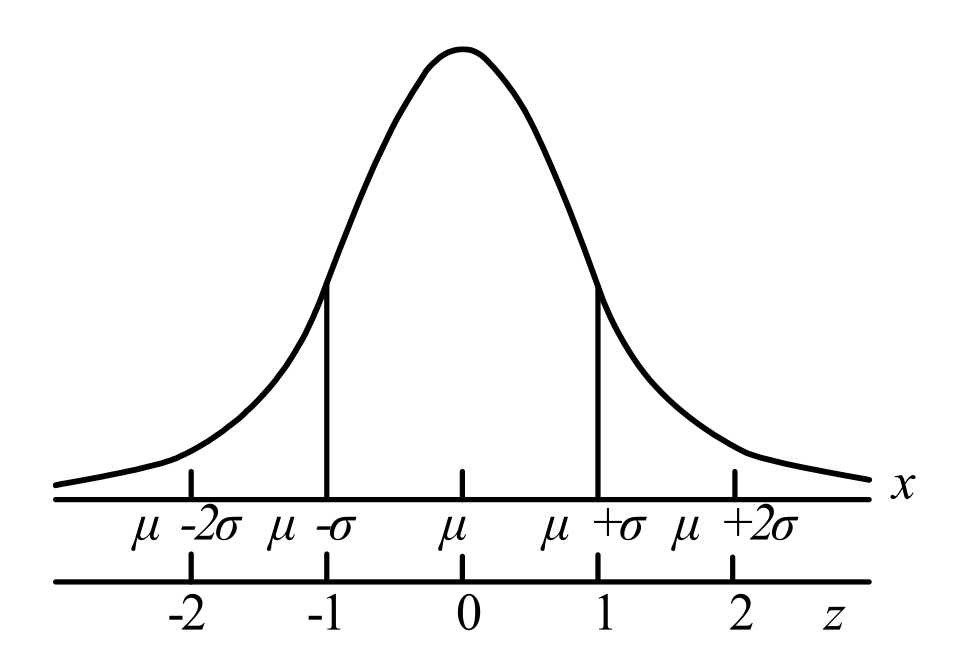
\includegraphics[width=0.5\textwidth]{fig//normal_dist.jpg}
	\caption{Distribution Function of Standard Normal Distribution}
\end{figure}

The total cholesterol of normal adult males aged 30 to 45 years follows a normal distribution. According to the standardization transformation:
\begin{equation}
	Z=\frac{X-\bar{x}}{s} = 0.91
\end{equation}

The percentage of normal adult males with total cholesterol greater than 5.72 mmol/L is the area to the right of the line $x=0.91$, and under the 
distribution function of standard normal distribution. According to the table of standard normal diatribution function, when $Z = 0.90588$,
the percentage is $18.14\%$. 
 
So $18.14\%$ of normal adult males have total cholesterol greater than 5.72mmol/L.

\section{Exercise 2}
\subsection{Sampling Error}
\begin{equation}
	sample \ size: n = 144
\end{equation}
\begin{equation}
	sampling \ error: s_{\bar{x}}=\frac{s}{\sqrt{n}} = 0.07 \ mmol/L
\end{equation}

\subsection{Confidence Interval}
\begin{equation}
	confidence \ interval : (\bar{x}-t_\alpha s_{\bar{x}},\bar{x}+t_\alpha s_{\bar{x}})
\end{equation}
\begin{equation}
	degree \ of \ freedom : v=n-1=143
\end{equation}

The $t_\alpha$ value corresponding to two sides probability $\alpha$.
According to the table of t distribution, $t_{0.05} = 1.980$ and $t_{0.01} = 2.617$ when $v=143$.

\begin{equation}
	95\% \ confidence \ interval \ (unit:mmol/L): (\bar{x}-t_{0.05} s_{\bar{x}},\bar{x}+t_{0.05} s_{\bar{x}})=(4.81,5.09)
\end{equation}
\begin{equation}
	99\% \ confidence \ interval \ (unit:mmol/L): (\bar{x}-t_{0.01} s_{\bar{x}},\bar{x}+t_{0.01} s_{\bar{x}})=(4.77,5.13)
\end{equation}

The $95\%$ confidence interval indicates that $95\%$ of the confidence intervals will include the population mean if we sample repestedly 
and use the same method to calculate the confidence interval. If we want a larger percentage of confidence intervals to include the population mean,
then a wider confidence interval is a necessity. As a result, the $99\%$ confidence interval is wider than the $95\%$ confidence interval. 
\end{document}